\chapter{Referencial Teórico}
Neste capítulo apresentaremos uma revisão da literatura agrupando trabalhos relacionados a reprovações e dificuldades de alunos em disciplinas de programação, novas abordagens de ensino e sistemas de dicas. 

\section{Reprovações em Disciplinas de Programação}

O entendimento e aplicação dos conceitos estudados em disciplinas de programação é fundamental para que o aluno consiga desenvolver programas mais complexo. \citeonline{Helminen:2010:JPV:1879211.1879234} afirmam que a programação é uma competência essencial no curso de Ciência da Computação. Segundo \citeonline{bosse2015reprovaccoes} os estudantes normalmente apresentam uma grande dificuldade com os conteúdos abordados, ocasionando em reprovação ou desistência.

\citeonline{Sinclair:2015:MSE:2729094.2742586} agruparam pesquisas internacionais como a \textit{National Survey of Student Engagement} (NSSE) feita na América do Norte e Canadá e a pesquisa \textit{Nacional Universidade Experience} (UES). Esse estudo reúne dados relacionadas à Ciência da Computação sendo que os resultados desta meta-análise indicam que o curso de Ciência da Computação apresenta taxas mais baixas do que a média em muitos dos principais pontos de referência de engajamento. 

A \cref{tabela:NSSEbenchmark} apresenta um resumo das pontuações dos indicadores do NSSE 2013 sendo o máximo de 60 pontos para cada indicador e quanto maior melhor. Assim, as pontuações do CBCC estão abaixo da média geral para todas as categorias exceto "Aprendizado Colaborativo" em que é igual. Em vários indicadores, o curso de Ciência da Computação está apenas 1 ou 2 pontos (em 60) atrás, mas em "Aprendizagem Reflexiva" e "Estratégias de Aprendizado" em particular, a diferença é maior. Em ambos esses indicadores as Ciências Físicas e Engenharia são geralmente de baixa pontuação e pode ser considerado como comparações sujeitas próximos do CBCC. 

\begin{table}[ht]
	\centering
	\captionsetup{justification=centering}
	\caption[Indicadores da pesquisa NSSE 2013]{Indicadores da pesquisa NSSE 2013. \\ Fonte: adaptada de \citeonline{Sinclair:2015:MSE:2729094.2742586}}
	\label{tabela:NSSEbenchmark}
	\begin{tabular}{|l|c|c|c|c|}
		\hline
		\textbf{Área da matéria}                                                  & \multicolumn{1}{l|}{\textbf{\begin{tabular}[c]{@{}l@{}}Ciência da \\ Computação\end{tabular}}} & \multicolumn{1}{l|}{\textbf{\begin{tabular}[c]{@{}l@{}}Ciências \\ Físicas\end{tabular}}} & \multicolumn{1}{l|}{\textbf{Engenharia}} & \multicolumn{1}{l|}{\textbf{No Geral}} \\ \hline
		\begin{tabular}[c]{@{}l@{}}Aprendizagem de \\ Ordem Superior\end{tabular} & 38                                                                                             & 40                                                                                        & 39                                        & 39                                     \\ \hline
		Aprendizagem Reflexiva                                                    & 32                                                                                             & 34                                                                                        & 33                                        & 39                                     \\ \hline
		Estratégias de Aprendizado                                                & 34                                                                                             & 39                                                                                        & 36                                        & 41                                     \\ \hline
		Raciocínio Quantitativo                                                   & 28                                                                                             & 38                                                                                        & 37                                        & 29                                     \\ \hline
		Aprendizado Colaborativo                                                  & 32                                                                                             & 36                                                                                        & 40                                        & 32                                     \\ \hline
		Qualidade das Interações                                                  & 42                                                                                             & 43                                                                                        & 41                                        & 43                                     \\ \hline
		Ambiente de Apoio                                                         & 31                                                                                             & 34                                                                                        & 32                                        & 33                                     \\ \hline
	\end{tabular}
\end{table}

A \cref{tabela:UESbenchmark} apresenta um resumo dos resultados da UES. Das categorias gerais nos UES, o CBCC apresenta mal resultados em duas: segundo mais baixo no "Desenvolvimento de Habilidades" em comparação dentro das 45 áreas específicas, e décimo mais baixo em "Qualidade de Ensino". Outras categorias apresentam melhores resultados, sendo uma acima da média para "Engajamento dos Alunos" e também "Suporte ao Estudante" e apenas dois abaixo da média para "Recurso de Aprendizagem".

\begin{table}[ht]
	\centering
	\captionsetup{justification=centering}
	\caption[Resumo dos resultados da UES]{Resumo dos resultados da UES. \\ Fonte: adaptada de \citeonline{Sinclair:2015:MSE:2729094.2742586}}
	\label{tabela:UESbenchmark}
	\begin{tabular}{|l|c|c|c|c|c|}
		\hline
		\multicolumn{1}{|c|}{\textbf{\begin{tabular}[c]{@{}c@{}}Área da \\ Matéria\end{tabular}}} & \textbf{\begin{tabular}[c]{@{}c@{}}Dev. de \\ habilidades\end{tabular}} & \textbf{\begin{tabular}[c]{@{}c@{}}Engajamento \\ dos Alunos\end{tabular}} & \textbf{\begin{tabular}[c]{@{}c@{}}Qualidade\\ de Ensino\end{tabular}} & \textbf{\begin{tabular}[c]{@{}c@{}}Recurso de \\ Aprendizagem\end{tabular}} & \textbf{\begin{tabular}[c]{@{}c@{}}Suporte ao \\ Estudante\end{tabular}} \\ \hline
		\begin{tabular}[c]{@{}l@{}}Ciência da \\ Computação\end{tabular}                          & 72                                                                                 & 58                                                                         & 74                                                                     & 81                                                                          & 54                                                                       \\ \hline
		No Geral                                                                                  & 79                                                                                 & 57                                                                         & 79                                                                     & 83                                                                          & 53                                                                       \\ \hline
	\end{tabular}
\end{table}

\section{Novas Técnicas de Ensino}

\citeonline{Knobelsdorf:2014:TTC:2538862.2538944} aplicaram uma abordagem cognitiva de aprendizagem no curso teórico realizado na Universidade de Potsdam, na Alemanha, e têm levado a uma redução significativa das taxas de falha do curso. O objetivo era tornar as práticas do curso teórico de Ciência da Computação mais visíveis aos alunos e, portanto, mais fáceis de adotar. Reforçaram a modelagem introduzindo uma sessão tutorial, que consiste em apresentar as habilidades para manusear e trabalhar com o conhecimento que os alunos devem desenvolver no curso. Aplicaram o método \textit{Scaffolding \& Fading}, onde foi oferecido exercícios preparatórios específicos que devem ser resolvidos em conjunto durante a sessão de exercícios e servem como preparação para o dever de casa. E por fim, forneciam \textit{feedback} para as submissões e trabalhos de casa realizados pelos alunos. Para avaliar a nova abordagem, foi realizado um exame final mantendo os mesmos requisitos das versões dos últimos 5 anos e foi obtido uma taxa de insucesso inferior a 10\% em dois anos consecutivos que antes alcançava de 30 a 60\%.

\citeonline{Cukierman:2015:PSU:2729094.2742623} realizou estudos experimentais para determinar se novas atividades em sala de aula, como a instrução entre pares e a aprendizagem ativa, auxiliada pelo uso de sistemas de resposta do público (\foreign{i-clickers}) utilizado em palestras e o Programa de Aperfeiçoamento Acadêmico (AEP), que consiste na intervenção pró-ativa centrada nos estudantes desenvolvida e gerida pela \foreign{School of Computing Science and Student Learning Commons} na Universidade \foreign{Simon Fraser}, proporcionando oportunidades de autorreflexão e exposição a estratégias de estudo melhoram em algumas medidas de resultado (tais como notas de exame final). Para realizar o experimento, foram definidas as seguintes variáveis:

\begin{itemize}
	\item \textbf{AEP}: Participação em atividades da AEP. Este é um preditor dicotômico que indica se os alunos participaram (codificados como 1) ou não (codificados como 0) nas atividades da AEP.
	
	\item \textbf{MID}: pontuações de meio termo. Este é um preditor contínuo, variando de 0 a 100.
	
	\item \textbf{WIC}: Participação ponderada do \foreign{I-clicker}. Este é um predictor contínuo que mede a participação do i-clicker que varia de 0 a 100 e calculado acumulando pontos de todas as conferências quando \foreign{i-clickers} foram usados. Nessas palestras, os pontos foram baseados incluindo a participação e resposta correta de perguntas no \foreign{i-clicker}.
	
	item \textbf{FIN:}: Pontuações finais do exame. Este é o critério contínuo ou variável de resultado, que varia de 0 a 100.
\end{itemize}

\begin{figure}[h]
	\centering
	\captionsetup{justification=centering}
	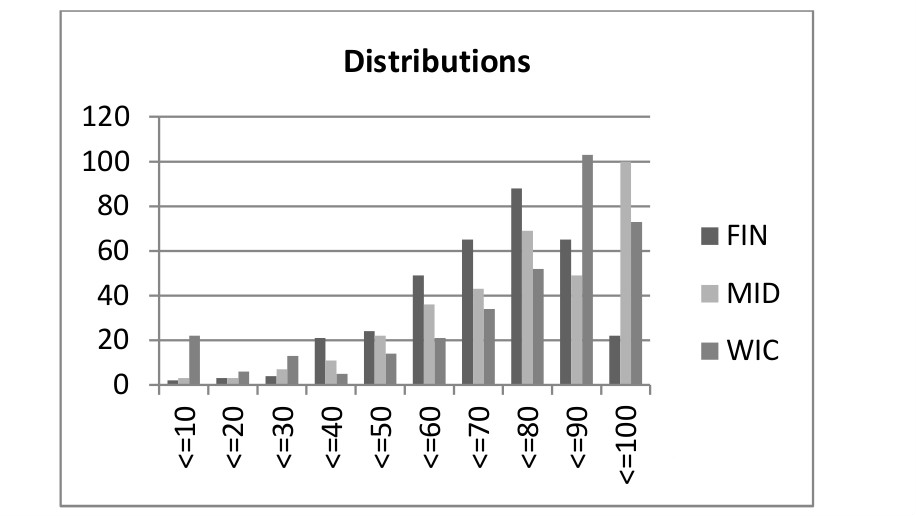
\includegraphics[width=.8\linewidth]{imagens/cukierman.png}
	\caption{Distribuições de FIN, MID e WIC. O gráfico não inclui os alunos que se retiraram do curso, nem com FIN = 0. \\ Fonte de \citeonline{Cukierman:2015:PSU:2729094.2742623}}
	\label{figura:resultadoCukierman}
\end{figure}

A \cref{figura:resultadoCukierman} a presenta o resultado obtido na pesquisa, sendo que o estudo não incluiu alunos que se retiraram do curso ou não vieram para o exame final. Intuitivamente, os alunos tiveram um desempenho muito bom no meio termo, com um grande número de alunos com mais de 90\%. Os alunos obtiveram valores muito bons nos pontos ponderados do \foreign{i-clicker} e no exame final pode-se observar que os resultados são mais distribuídos, embora negativamente inclinados.

\citeonline{Edwards:2015:ECI:2729094.2742632} abordam o problema da procastinação que é um problema generalizado que afeta significativamente os alunos do curso avançado de estruturas de dados de nível júnior. Muitos educadores de informática descrevem a procastinação como um dos problemas mais comuns que levam ao insucesso no curso. Teoriza-se que a procrastinação tem uma impacto sobre o desempenho dos alunos. De acordo com uma meta-análise de uma ampla gama de estudos de procrastinação, entre 70\% e 95\% dos estudantes de graduação procrastinam suas atividades em cursos de primeiro grau. 

Portanto, os pesquisadores investigaram três intervenções na sala de aula que são viáveis para os instrutores e que demanda pouco tempo: a reflexão ativa escrevendo tarefas, onde os alunos escrevem um "papel minucioso" após cada atribuição sobre suas escolhas de gerenciamento de tempo afetaram seu trabalho; Planilhas de planejamento preenchidas pelos alunos, exigindo-lhes quebrar as tarefas e mostrar quanto tempo eles planejam alocar para cada uma,  ajudando-os a formar, expressar, gerenciar e controlar os prazos em menor escala; E alertas por e-mail de consciência situacional baseados em um modelo de progresso do aluno que mostram cada aluno como seus esforços atuais comparado com as expectativas para a classe como um todo. Das intervenções estudadas, as atribuições de escrita reflexiva não produziram evidências de qualquer impacto significativo nas atividades do aluno. No entanto, mudanças na intervenção, como fazer com que os alunos discutam suas reflexões, talvez usando uma atividade de aprendizagem de pares poderia melhorar a sua eficácia. 

Da mesma forma, as atribuições de folha de cronograma também não produziram evidência consistente para um impacto significativo. Este estudo indica que os alertas de alerta de situação de e-mail mostraram uma redução estatisticamente significativa nas submissões tardias (23\% menos na média), bem como um aumento estatisticamente significativo na conclusão precoce (31\% mais em média) em comparação com o grupo de controle. Por causa da natureza de estudos como este, no entanto, existe o risco de outros fatores também terem desempenhado um papel, como diferenças nas populações estudantis, diferenças nas atribuições ou diferenças nos prazos das classes concorrentes em outros cursos.

\section{Mecanismo de Dicas}

Nas abordagens citadas a baixo, uma dica equivale a um auxílio ao aluno para que ele consiga realizar um exercício que esteja com dificuldade, essa dica pode ser oferecida tanto pelo professor ou colega de turma. Um sistema que utiliza esse conceito pode ser chamado de sistema de dicas, onde reproduz esse contato que o aluno teria com uma pessoa mais instruída quando precisa tirar uma dúvida ou pedir uma dica para realizar o exercício. Mas o aluno com dificuldades não pode ter esse apoio todo o tempo, então estão sendo criados sistema de dicas para suprir essa necessidade de auxiliar o aluno no seu aprendizado.

\citeonline{Elkherj:2014:SSR:2556325.2567864} apontam que as sugestões utilizadas em sistemas de aprendizagem on-line para ajudar os alunos quando eles estão tendo dificuldades são fixados antes do tempo e não dependem das tentativas mal sucedidas que o aluno já fez. Isto limita severamente a eficácia das sugestões. Eles desenvolveram um sistema alternativo para dar dicas aos estudantes. A principal diferença é que o sistema permite um instrutor enviar uma dica para um estudante após o aluno ter feito várias tentativas para resolver o problema e falhou. Depois de analisar os erros do aluno, o instrutor é mais capaz de entender o problema no pensamento do aluno e enviar-lhes uma dica mais útil. O sistema foi implantado em um curso de probabilidade e estatística com 176 alunos, obtendo \foreign{feedback} dos alunos muito positivo. Mas o desafio que os autores enfrentam é como escalar efetivamente o sistema de forma que todos os alunos que precisam de ajuda obtenham dicas eficazes. Pois com uma grande quantidade de alunos ficaria exaustivo para os instrutores avaliarem cada submissão dos exercícios de cada aluno para retornarem uma dica especifica do erro cometido. Então eles criaram um banco de dados de dica que permite que os instrutores reutilizem, compartilhem e melhorem em cima de sugestões escritas anteriormente.

\citeonline{Price:2015:IIF:2787622.2787748} está utilizando um sistema de tutores inteligentes (STI) que podem manter os alunos no caminho certo, na ausência de instrutores, fornecendo sugestões e advertências para os alunos que precisam de ajuda. Além disso, as técnicas baseadas em dados podem gerar feedback automaticamente a partir de tentativas de resolução de um problema. O autor está aplicando o seu estudo permitindo que os alunos escrevam códigos que se conectam com seus interesses, tais como jogos, aplicações e histórias. Como exemplo concreto, imagine um aluno que esteja desenvolvendo um jogo simples, quer requer a utilização de variáveis, laços de repetição, condicionais. Mas o aluno está com dificuldades em relação a uma funcionalidade que o jogo terá, ele poderá pedir uma dica para implementar essa funcionalidade que será gerada automaticamente pelo sistema com relação as tentativas anteriores de outros alunos.

\citeonline{Cummins:2016:IUH:2876034.2893379} investigaram  o uso de dicas para 4.652 usuários qualificados em um ambiente de aprendizagem on-line de grande escala chamado Isaac, que permite aos usuários para responder a perguntas de física com até cinco dicas. Foi investigado o comportamento do usuário ao usar dicas, engajamento dos usuários com desvanecimento (o processo de tornar-se gradualmente menos dependentes das dicas fornecidas), e estratégias de dicas incluindo decomposição, correção, verificação ou comparação. Como resultados obtidos, os alunos apresentaram estratégias para as resoluções dos exercícios sendo a mais comum é ver o conceito da dica para realizar a decomposição do problema e, em seguida, enviar uma resposta correta. A outra estratégia é usar os conceitos da dica para determinar se a pergunta pode ser respondida, uma grande proporção dos usuários que utilizaram essa estratégia acabou não tentando responder a pergunta

\citeonline{Glassman:2016:LPH:2818048.2820011} criaram um sistema de dicas chamado \foreign{Dear Beta} para auxiliar projetos de circuitos digitais que exigem mais experiência dos alunos, assim aplicando o método do \foreign{learnersourcing} os alunos apresentaram mais motivação para se envolver no conteúdo de apendizagem, mas também se beneficiaram podagogicamente da próproa tarefa de realizar exercícios e produzir dicas. No estudo realizado pelos pesquisadores, nove dos 226 alunos do curso de arquitetura de computadores participaram do estudo. Estes alunos foram recrutados através de um forúm. Os participantes receberam US \$30 para realizarem o estudo, que durou uma hora. Esse estudo foi realizado para estudar a eficácia das dicas para otimizar os circuitos para que usassem menos transistores. 

Após algumas semanas de estudo o número de voluntários aumentou e chegou a 20 alunos, mas na últma semana de acabar o estudo o número de usuários registrados no sistema \foreign{Dear Beta} aumentou linearmente de 20 para 166. Nos 9 dias entre o lançamento do \foreign{Dear Beta} e a data de vencimento do estudo de laboratório, os usuários adicionaram 76 erros de verificação e 57 sugestões como uma resposta a esses erros. Metade dos erros recebeu pelo menos uma dica. O Beta e Dear Gamma, que aplicam os fluxos de trabalho à criação de dicas de depuração e otimização, combinando os alunos com a tarefa de criação de dica, considerando seu progresso atual. Os resultados do estudo de implantação e subsequente estudo de laboratório demonstram a viabilidade desses fluxos de trabalho e indicam que as dicas geradas pelo aluno são úteis para os alunos. 

\section{Considerações Finais}

Muitos pesquisadores estão estudando e aplicando diferentes estratégias para melhorar o ensino de programação, minimizar reprovações e desistências dos alunos em cursos de computação. Nosso estudo irá adotar como base para a criação do sistema de dicas o estudo realizado por \citeonline{Glassman:2016:LPH:2818048.2820011}, que desenvolveu um sistema de dicas para auxiliar projetos de circuitos digitais no curso de arquitetura de computadores. Queremos construir um sistema que difere do apresentado por \citeonline{Elkherj:2014:SSR:2556325.2567864}, onde o professor apresenta uma dica em tempo real a um aluno que tenha realizado várias tentativas para resolver um exercício, esse tipo de sistema não é escalavél para uma grande quantidade de usuários. Nosso objetivo é criar um sistema o qual não seja necessário que um professor ou instrutor criem dicas para os alunos, queremos que os próprios alunos criem dicas para ajudar outros colegas e melhorem seu desempenho em programação.